\documentclass[12pt]{article}

\usepackage[utf8]{inputenc}
\usepackage{datetime}
\usepackage{amsthm}
\usepackage{amsmath}
\usepackage{amssymb}
\usepackage{enumitem}
\usepackage[USenglish]{babel}
\usepackage{matlab-prettifier}
\usepackage{graphicx}
\usepackage[makeroom]{cancel}
\usepackage{afterpage}
\usepackage{capt-of}

\DeclareMathOperator*{\argmin}{arg\,min}

\newcommand\independent{\protect\mathpalette{\protect\independenT}{\perp}}
\def\independenT#1#2{\mathrel{\rlap{$#1#2$}\mkern2mu{#1#2}}}

\newtheoremstyle{colon}{\topsep}{\topsep}{}{}{\bfseries}{:}{ }{}
\theoremstyle{colon}
\newtheorem{exercise}{Exercise}
\newtheorem*{answer}{Answer}

\title{ORFE 525: Statistical Learning and Nonparametric Estimation \\ Homework 1}
\author{Zachary Hervieux-Moore \\ Collaborator: Guillaume Martinet}

\newdate{date}{09}{03}{2017}
\date{\displaydate{date}}

\begin{document}

\maketitle

\clearpage

\begin{exercise}
  Complete the following in R. The goal is to predict house price from a dataset.
  \begin{enumerate}[label=\arabic*)]
    \item Convert the \texttt{zipcode} column into factors, and discuss why this conversion is necessary if we want to use the \texttt{zipcode} column as an explanatory variable in linear regression.
      (Hint: Factors are how R represents indicator variables. You can do this with \texttt{as.factor()}.)

    \item Build a linear model on the training data using \texttt{lm()} by regressing the housing price on these variables: \texttt{bedrooms}, \texttt{bathrooms}, \texttt{sqft\_living}, and \texttt{sqft\_lot}.
      \begin{enumerate}[label=\alph*)]
        \item What's the $R^2$ of the model on the training data? What's the $R^2$ on the testing data?
        \item What if we want to use the \texttt{zipcode} to explain/predict the housing price? Add zipcode in your linear model, does it improve the $R^2$ or prediction power?
      \end{enumerate}

    \item Fit the model on the training data using the \texttt{glmnet} function to predict the house prices using all the 18 features (columns on the right of the \texttt{price} column).
      \begin{enumerate}[label=\alph*)]
        \item Plot the regularization paths of Lasso and Ridge (both have L1 norm as the x-axis). Based on the 2 graphs you just plotted, which features seem to be more important than others?
          (\textbf{Note:} You may choose your own criteria for how to identify important features. However, you must explain these choices clearly in your write-up.)
        \item For both Lasso and Ridge regression, use a 5-fold cross validation (via the \texttt{cv.glmnet} function) to determine the tuning parameter $\lambda$. Mark the corresponding L1-norm on your plot made in Part a). Also plot the cross validation (use log($\lambda$) as the x-axis). (\textbf{Hint:} Use \texttt{model.matrix} to implement categorical variables in \texttt{glmnet})
        \item Evaluate both models by using the testing data. Record mean squared test error.
      \end{enumerate}

    \item Fit the model on the training data using the \texttt{randomForest} function to predict the house prices using the features \texttt{sqft\_living}, \texttt{sqft\_lot}, \texttt{bedrooms}, \texttt{bathrooms}, \texttt{floors}, and \texttt{zipcode}. Plot variable importance for the variables (via \texttt{varImpPlot}). Use \texttt{partialPlot} to plot the partial dependence for the top three variables in variable importance.
      (\textbf{Note:} Random forest cannot handle a categorical variable with more than 32 categories. Please find a meaningful way to regroup the zipcode numbers.)

    \item Guess the price of Donald Trump's house (using the data provided) using the most reasonable model you think above. Do you think the predicted price is reasonable?
  \end{enumerate}
\end{exercise}

\begin{answer}
  The code used to generate all theses answers are appended at the end of the question.
  \begin{enumerate}[label=\arabic*)]
    \item It is necessary to convert the column because if you regressed on the \texttt{zipcode} column without doing so, it would fit $\beta$ to the the actual zipcode number. That is, something like
      \begin{gather*}
        price = \beta_0 + \beta_1 * zipcode + \mathellipsis
      \end{gather*}
      Obviously, one could do this, but the meaning is questionable. Houses are not linearly related to zipcode. That is, as one increases zipcodes, the price of houses could go up and down. That is Beverly Hills (90210) and New York City (10012) are certainly more expensive than than Topeka, Kansas (66621) but Topeka is between the two values. Using factors corrects this by turning zipcode into many binary indicators. Which makes the regression
      \begin{gather*}
        price = \beta_0 + \beta_1 \cdot 1_{\{zipcode=44444\}} + \beta_2 \cdot 1_{\{zipcode=44445\}} + \mathellipsis
      \end{gather*}
      Thus, this models how zipcodes can add or subtract value depending on whether the house is in the zipcode or not.

    \item
      \begin{enumerate}[label=\alph*)]
        \item The $R^2$ of the linear model on the training data is 0.5101. The $R^2$ for the testing data is 0.5051.
        \item After adding the zipcode, the $R^2$ of the linear model on the training data is 0.7393. The $R^2$ for the testing data is 0.7380. Which shows that it improves the $R^2$ and prediction power by a signficant amount. Also, we never expect that adding more variables decreases the $R^2$ because, if it did, we could just set the new variable $\beta$ parameter to be 0 and get the previous $R^2$.
      \end{enumerate}

    \item
      \begin{enumerate}[label=\alph*)]
        \item The two regularization paths are below. Note, there are many lines because I turned the zipcodes into indicator variables as per question 1.1. In the regularization paths, we are looking for the first variables to get an active $\beta$ parameter at low $\lambda$ values. This indicates that it has the strongest effect. Thus, the Ridge path is not too useful as all the parameters seem to diverge at 0. However, the Lasso path is more sporadic. Lasso suggests that different zipcodes are significant which makes sense. Also, waterfront, square footage of living space, and grade are also significant by this criteria.

          \begin{center}
            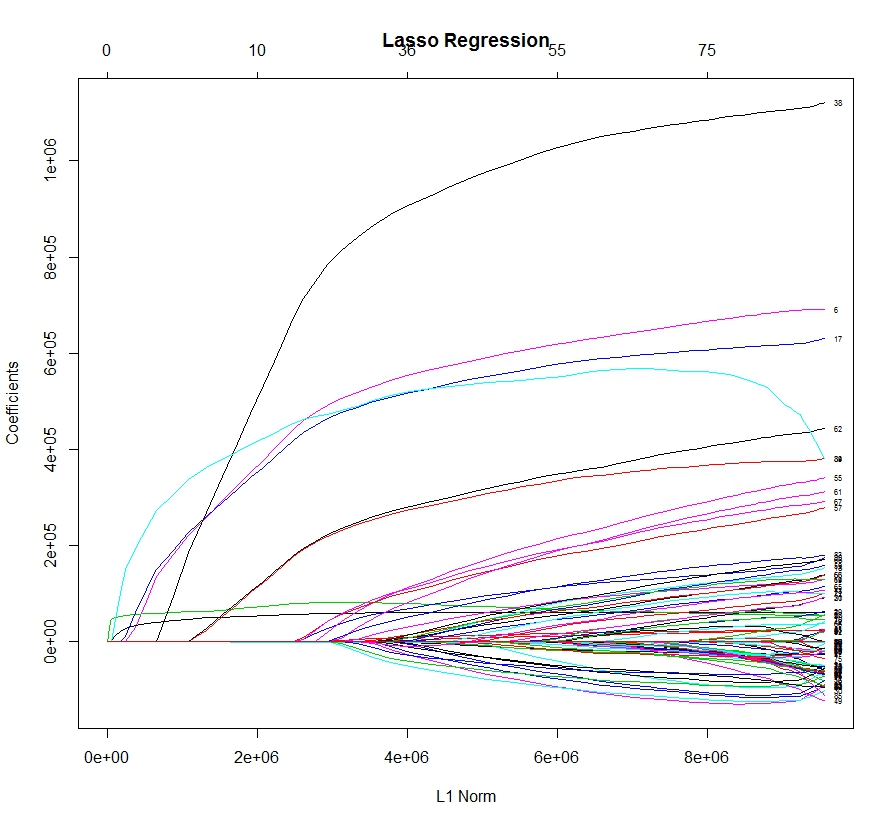
\includegraphics[width=0.8\textwidth]{13a_lasso.jpg}
            \captionof{figure}{Lasso Regularization Path}
          \end{center}

          \begin{center}
            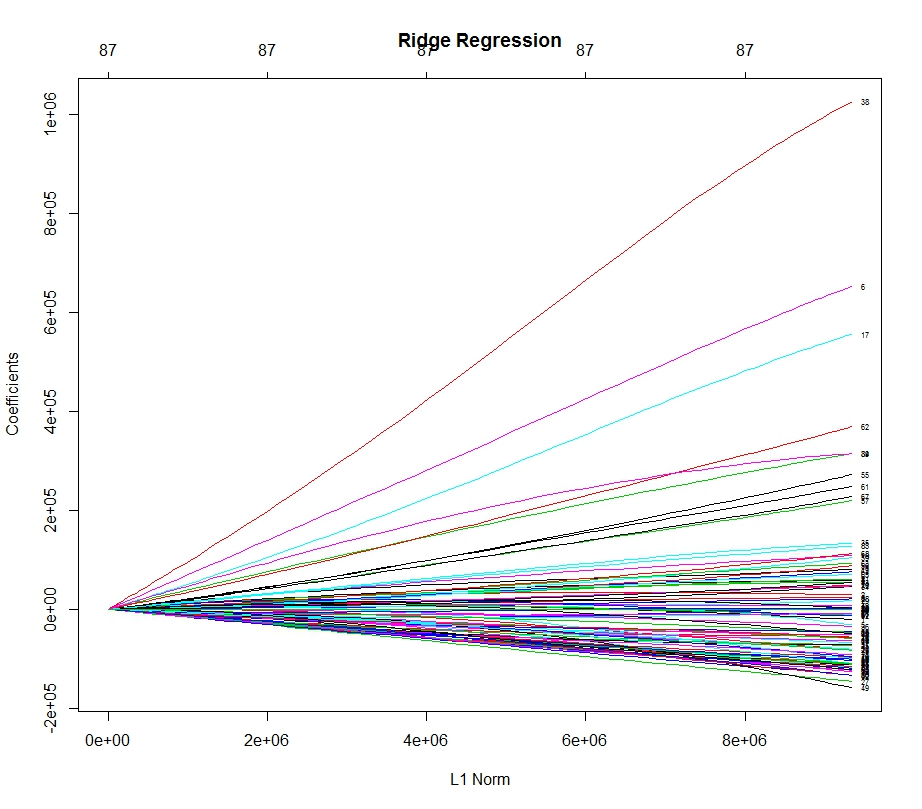
\includegraphics[width=0.8\textwidth]{13a_ridge.jpg}
            \captionof{figure}{Ridge Regularization Path}
          \end{center}

        \item After doing the 5-fold cross validation, the tuning parameter $\lambda$ is 182.16 for Lasso and 28337.98 for Ridge. The corresponding norm value are shown as the solid black vertical lines in the first two figures below. The cross validation plots are shown after.

          \begin{center}
            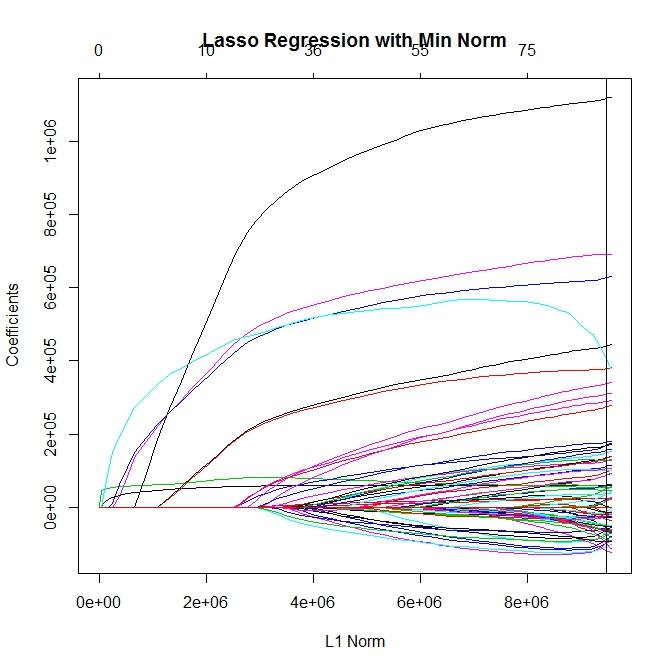
\includegraphics[width=0.8\textwidth]{13b_lasso_min.jpg}
            \captionof{figure}{Lasso Regularization Path with Min Lambda Norm}
          \end{center}

          \begin{center}
            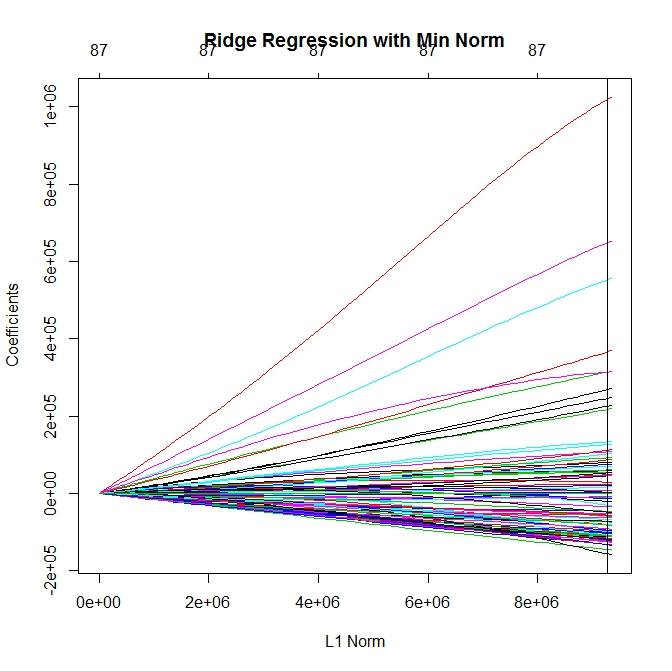
\includegraphics[width=0.8\textwidth]{13b_ridge_min.jpg}
            \captionof{figure}{Ridge Regularization Path with Min Lambda Norm}
          \end{center}

          \begin{center}
            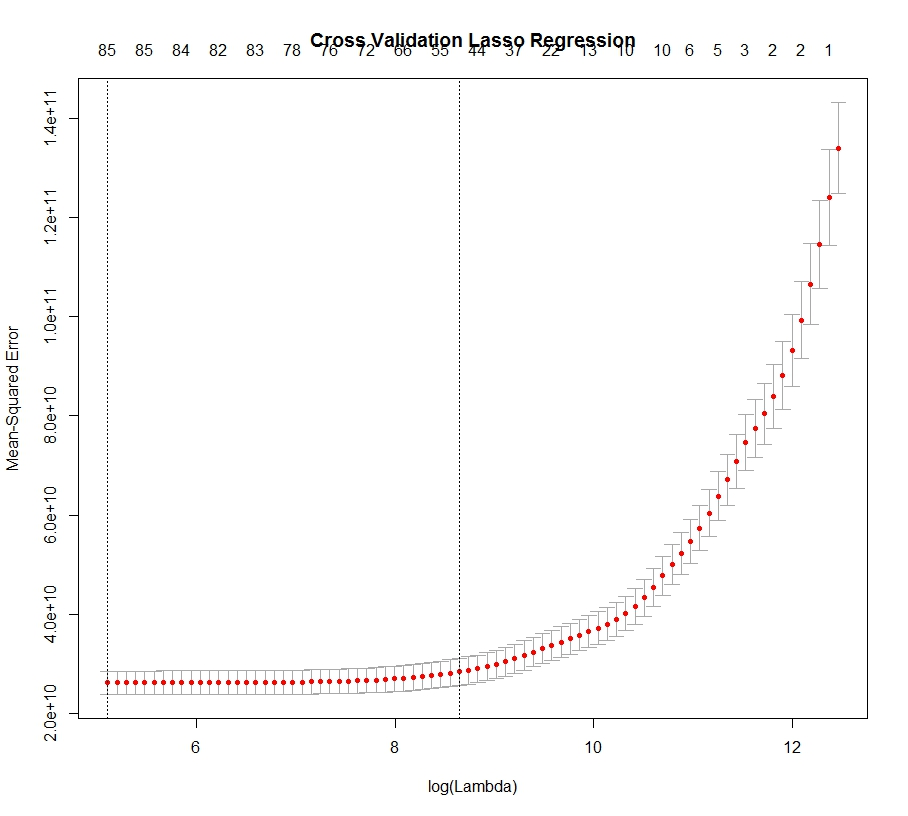
\includegraphics[width=0.8\textwidth]{13b_lasso_cv.jpg}
            \captionof{figure}{Lasso Cross Validation}
          \end{center}

          \begin{center}
            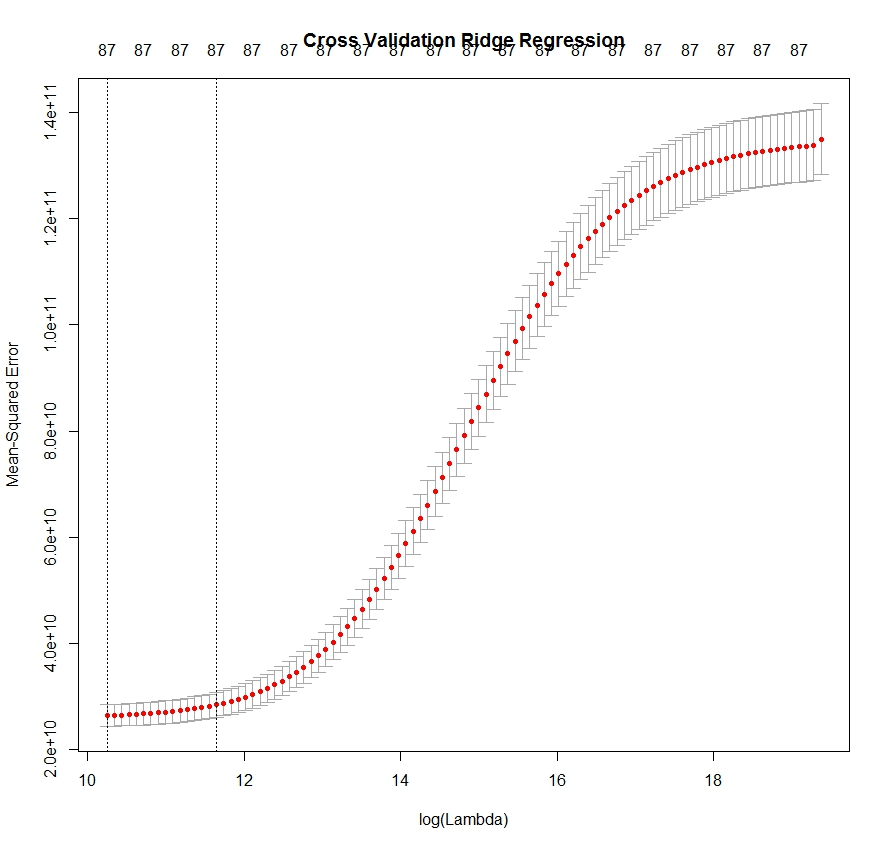
\includegraphics[width=0.8\textwidth]{13b_ridge_cv.jpg}
            \captionof{figure}{Ridge Cross Validation}
          \end{center}

        \item Evaluating both models on the test data, the Lasso regression has an $R^2$ of 0.8002 and Ridge regression has an $R^2$ of 0.8004. The mean squared test error for Lasso is 26822892590 and the mean squared test error for Ridge is 26854501856. These numbers may seem high given that the $R^2$ is pretty good. But given the size of the data set, a few outliers (undervalued expensive houses) could cause that much error.
      \end{enumerate}

    \item The plots for the importance of the variables and the partial dependence for the random forest are shown below. To handle the zipcode issue, I kept the leading 3 digits of the zipcode. This reduced the number of factors but kept the meaningfulness of the zipcode since each zipcodes that are close to each other tend to be close to each other geographically.

      \begin{center}
        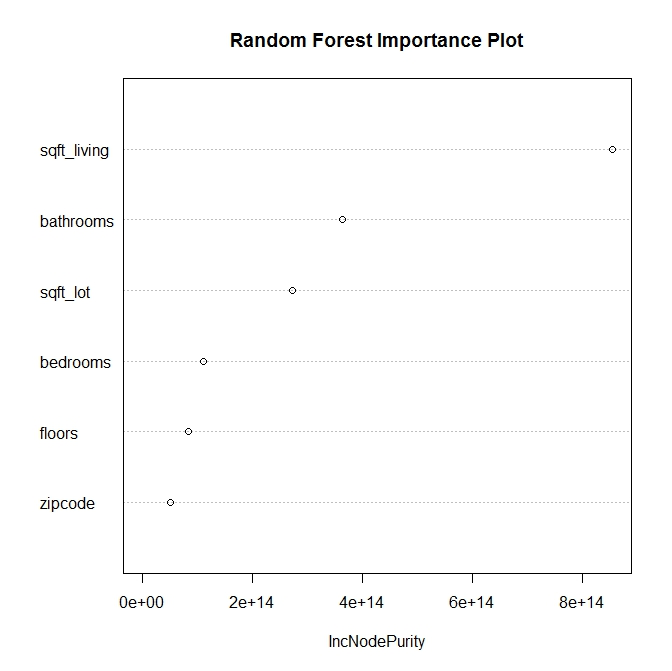
\includegraphics[width=0.8\textwidth]{14_important.jpg}
        \captionof{figure}{Variable Importance}
      \end{center}

      \begin{center}
        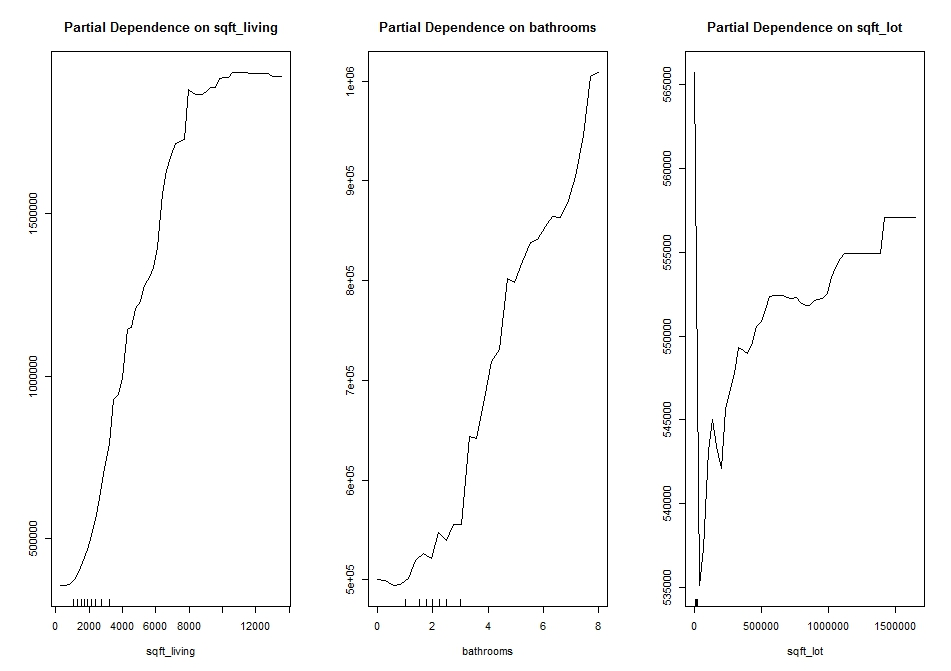
\includegraphics[width=0.8\textwidth]{14_partial.jpg}
        \captionof{figure}{Partial Dependence for sqft\_living, bathrooms, and sqft\_lot}
      \end{center}

    \item The most reasonable model developed was the Ridge regression as this had the highest $R^2$ value. But also, the random forest is not very good at extrapolating since it is based on making regions in the sample space. Thus, if you give a random forest a sample to estimate that it hasn't seen before, it will group it with the closest samples it has data on. Since Trump's house is no where near any house on the list, it is best not to use random forest. The Ridge regression predicts a house value of \$11.3M. This is definitely in the right order of magnitude. However, given that the latitude and longitude point exactly to Bill Gates' house, I doubt that his house is only worth \$11.3M.
  \end{enumerate}

  \textbf{Code Appendix}

  \begin{lstlisting}[language=R, basicstyle=\scriptsize, breaklines=true]
    train <- read.csv('train.data.csv')
    test <- read.csv('test.data.csv')

    # Part 1.1 - Turn zipcode into factors
    train$zipcode <- factor(train$zipcode)
    test$zipcode <- factor(test$zipcode)

    # Part 1.2a - Fit linear model
    train.lm <- lm(price ~ bedrooms + bathrooms + sqft_living + sqft_lot, data=train)
    print("R squared for training set:")
    summary(train.lm)$r.squared
    test.pred <- predict(train.lm, newdata=test)

    ## R squared for prediction (square of correlation)
    print("R squared for test set:")
    cor(test$price, test.pred)^2

    # Part 1.2b - Fit linear model with zipcode
    train.lm <- lm(price ~ bedrooms + bathrooms + sqft_living + sqft_lot + zipcode, data=train)
    print("R squared for training set:")
    summary(train.lm)$r.squared
    test.pred <- predict(train.lm, newdata=test)

    ## R squared for prediction (square of correlation)
    print("R squared for test set:")
    cor(test$price, test.pred)^2

    # Part 1.3a - Fit glmnet and plot regularization paths
    library(glmnet)

    ## Lasso regression
    train.glm.lasso <- glmnet(model.matrix(~ 0 + bedrooms + bathrooms + sqft_living + sqft_lot + floors + waterfront + view + condition + grade + sqft_above + sqft_basement + yr_built + yr_renovated + zipcode + lat + long + sqft_living15 + sqft_lot15, data=train), data.matrix(train$price), alpha=1)
    plot(train.glm.lasso, label=TRUE)
    title(main="Lasso Regression")

    ## Ridge regression
    train.glm.ridge <- glmnet(model.matrix(~ 0 + bedrooms + bathrooms + sqft_living + sqft_lot + floors + waterfront + view + condition + grade + sqft_above + sqft_basement + yr_built + yr_renovated + zipcode + lat + long + sqft_living15 + sqft_lot15, data=train), data.matrix(train$price), alpha=0)
    dev.new()
    plot(train.glm.ridge, label=TRUE)
    title(main="Ridge Regression")

    # Part 1.3b - Cross validation
    train.glm.lasso.cv <- cv.glmnet(model.matrix(~ 0 + bedrooms + bathrooms + sqft_living + sqft_lot + floors + waterfront + view + condition + grade + sqft_above + sqft_basement + yr_built + yr_renovated + zipcode + lat + long + sqft_living15 + sqft_lot15, data=train), data.matrix(train$price), alpha=1, nfolds=5)
    print("Lambda min for lasso:")
    train.glm.lasso.cv$lambda.min
    dev.new()
    plot(train.glm.lasso.cv)
    title(main="Cross Validation Lasso Regression")

    ## Looked manually to figure out min lasso index
    print("Beta min for lasso:")
    train.glm.lasso.cv$glmnet.fit$beta[,"s67"]
    print("Beta min l_1 norm:")
    norm(as.matrix(train.glm.lasso.cv$glmnet.fit$beta[,"s67"]), type="1")

    ## Plot min norm
    dev.new()
    plot(train.glm.lasso.cv$glmnet.fit)
    abline(v=train.glm.lasso.cv$lambda.min)
    title(main="Lasso Regression with Min Norm")

    train.glm.ridge.cv <- cv.glmnet(model.matrix(~ 0 + bedrooms + bathrooms + sqft_living + sqft_lot + floors + waterfront + view + condition + grade + sqft_above + sqft_basement + yr_built + yr_renovated + zipcode + lat + long + sqft_living15 + sqft_lot15, data=train), data.matrix(train$price), alpha=0, nfolds=5)
    print("Lambda min for ridge:")
    train.glm.ridge.cv$lambda.min
    dev.new()
    plot(train.glm.ridge.cv)
    title(main="Cross Validation Ridge Regression")

    ## Looked manually to figure out min ridge index
    print("Beta min for ridge:")
    train.glm.ridge.cv$glmnet.fit$beta[,"s99"]
    print("Beta min l_1 norm:")
    norm(as.matrix(train.glm.ridge.cv$glmnet.fit$beta[,"s99"]), type="1")

    ## Plot min norm
    dev.new()
    plot(train.glm.ridge.cv$glmnet.fit)
    abline(v=train.glm.ridge.cv$lambda.min)
    title(main="Ridge Regression with Min Norm")

    # Part 1.3c - Evaluate models
    test.glm.lasso.pred <- predict(train.glm.lasso.cv, newx=model.matrix(~ 0 + bedrooms + bathrooms + sqft_living + sqft_lot + floors + waterfront + view + condition + grade + sqft_above + sqft_basement + yr_built + yr_renovated + zipcode + lat + long + sqft_living15 + sqft_lot15, data=test), s="lambda.min")
    print("Mean squared error of Lasso prediction:")
    sum((test$price - test.glm.lasso.pred)^2)/length(test.glm.lasso.pred)
    print("R squared for test set:")
    cor(test$price, test.glm.lasso.pred)^2

    test.glm.ridge.pred <- predict(train.glm.ridge.cv, newx=model.matrix(~ 0 + bedrooms + bathrooms + sqft_living + sqft_lot + floors + waterfront + view + condition + grade + sqft_above + sqft_basement + yr_built + yr_renovated + zipcode + lat + long + sqft_living15 + sqft_lot15, data=test), s="lambda.min")
    print("Mean squared error of Ridge prediction:")
    sum((test$price - test.glm.ridge.pred)^2)/length(test.glm.ridge.pred)
    print("R squared for test set:")
    cor(test$price, test.glm.ridge.pred)^2

    # Part 1.4 - Random Forest
    library(randomForest)

    ## zipcode needs to be changed, leading digits highly meaningful to specific region of US
    train$zipcode <- substr(train$zipcode,1,3)
    test$zipcode <- substr(test$zipcode,1,3)
    train.randomforest <- randomForest(price ~ sqft_living + sqft_lot + bedrooms + bathrooms + floors + zipcode, data=train)
    dev.new()
    varImpPlot(train.randomforest, main="Random Forest Importance Plot")

    ## Plot partial dependence of top 3 important variables
    dev.new()
    train.randomforest.imp <- importance(train.randomforest)
    train.randomforest.imp <- train.randomforest.imp[order(train.randomforest.imp, decreasing=TRUE),]
    train.randomforest.imp <- train.randomforest.imp[1:3]
    train.randomforest.impvar <- names(train.randomforest.imp)
    op <- par(mfrow=c(1, 3))
    for (i in seq_along(train.randomforest.impvar)) {
      partialPlot(train.randomforest, train, train.randomforest.impvar[i], xlab=train.randomforest.impvar[i], main=paste("Partial Dependence on", train.randomforest.impvar[i]))
    }
    par(op)

    ## Calculate R squared
    test.randomforest.pred <- predict(train.randomforest, newdata=test)
    print("R squared for test set:")
    cor(test$price, test.randomforest.pred)^2

    # Part 1.5 - Trump

    ## Reload data to ensure integrity from zipcode change

    train <- read.csv('train.data.csv')
    test <- read.csv('test.data.csv')

    train$zipcode <- factor(train$zipcode)
    test$zipcode <- factor(test$zipcode)

    donald_trump = data.frame(X=1, id=1, date='20141013T000000', price=14000000,
      bedrooms=8, bathrooms=25, sqft_living=50000,
      sqft_lot=225000, floors=4, zipcode=factor(c('98039')), condition=10, grade=10,
      waterfront=1, view=4, sqft_above=37500, sqft_basement=12500, yr_built=1994,
      yr_renovated=2010, lat=47.627606, long=-122.242054, sqft_living15=5000,
      sqft_lot15=40000)
    ## Make large test set for model.matrix to generate right matrix for Trump
    donald_trump_matrix <- rbind(test, donald_trump)

    predict(train.lm, newdata=donald_trump)
    predict(train.glm.lasso.cv, newx=model.matrix(~ 0 + bedrooms + bathrooms + sqft_living + sqft_lot + floors + waterfront + view + condition + grade + sqft_above + sqft_basement + yr_built + yr_renovated + zipcode + lat + long + sqft_living15 + sqft_lot15, data=donald_trump_matrix), s="lambda.min")[length(donald_trump_matrix[,1]),]
    predict(train.glm.ridge.cv, newx=model.matrix(~ 0 + bedrooms + bathrooms + sqft_living + sqft_lot + floors + waterfront + view + condition + grade + sqft_above + sqft_basement + yr_built + yr_renovated + zipcode + lat + long + sqft_living15 + sqft_lot15, data=donald_trump_matrix), s="lambda.min")[length(donald_trump_matrix[,1]),]
    donald_trump$zipcode <- substr(donald_trump$zipcode,1,3)
    predict(train.randomforest, newdata=donald_trump)
  \end{lstlisting}
\end{answer}

\clearpage

\begin{exercise}
  The Lasso usually does not have an explicit formula for its solution. However, in this problem, you will be lucky enough as we are considering a very special case.

  Let $\theta \in \mathbb{R}^d$ and $Y \in \mathbb{R}^d$. For any $\tau > 0$, we define the hard thresholding $\hat{\theta}^{HRD}$ and the soft thresholding $\hat{\theta}^{SFT}$ as
  \begin{gather*}
    \hat{\theta}_j^{HRD} = \begin{cases}
      Y_j & \text{if } \lvert Y_j \rvert > 2 \tau \\
      0 & \text{if } \lvert Y_j \rvert \leq 2 \tau
    \end{cases} \text{ and } \hat{\theta}_j^{SFT} = \begin{cases}
      Y_j - 2 \tau & \text{if } Y_j > 2 \tau \\
      0 & \text{if } \lvert Y_j \rvert \leq 2 \tau \\
      Y_j + 2 \tau & \text{if } Y_j < -2 \tau
    \end{cases}
  \end{gather*}
  for $j = 1, \mathellipsis, d$. Define $\lVert \theta \rVert_0 = \lvert \{ j : \theta_j \neq 0 \} \rvert$, where for any set $S$, $\lvert S \rvert$ is the cardinality of $S$. Proce that
  \begin{gather*}
    \hat{\theta}_j^{HRD} = \argmin_{\theta \in \mathbb{R}^d} \{ \lVert Y - \theta \rVert_2^2 + 4 \tau^2 \lVert \theta \rVert_0 \}, \\
    \hat{\theta}_j^{SFT} = \argmin_{\theta \in \mathbb{R}^d} \{ \lVert Y - \theta \rVert_2^2 + 4 \tau \lVert \theta \rVert_1 \}
  \end{gather*}
\end{exercise}

\begin{answer}
  First, let us work with $\hat{\theta}_j^{HRD}$. Expand the norm,
  \begin{gather*}
    \argmin_{\theta \in \mathbb{R}^d} \lVert Y - \theta \rVert_2^2 + 4 \tau^2 \lVert \theta \rVert_0 \\
    = \argmin_{\theta \in \mathbb{R}^d} Y^T Y - 2 Y^T \theta + \theta^T \theta + 4 \tau^2 \lVert \theta \rVert_0
  \end{gather*}
  We drop the term that has no $\theta$ dependence
  \begin{gather*}
    = \argmin_{\theta \in \mathbb{R}^d} - 2 Y^T \theta + \lVert \theta \rVert_2^2 + 4 \tau^2 \lVert \theta \rVert_0 \\
    = \argmin_{\theta \in \mathbb{R}^d} \sum_{j=1}^d - 2 Y_j^T \theta_j + \theta_j^2 + 4 \tau^2 \cdot 1_{\{\theta_j \neq 0\}}
  \end{gather*}
  Thus, we can just minimize each component individually.
  \begin{gather}
    = \argmin_{\theta \in \mathbb{R}^d} - 2 Y_j \theta_j + \theta_j^2 + 4 \tau^2 \cdot 1_{\{\theta_j \neq 0\}}
  \end{gather}
  We lower bound this by taking the absolute values of $Y_j$ and $\theta_j$ as this can only reduce the min.
  \begin{gather*}
    \geq \argmin_{\theta \in \mathbb{R}^d} - 2 \lvert Y_j \rvert \lvert \theta_j \rvert + \theta_j^2 + 4 \tau^2 \cdot 1_{\{\theta_j \neq 0\}}
  \end{gather*}
  Case 1, suppose that $\lvert Y_j \rvert \leq 2 \tau$. Then we can lower bound even further
  \begin{gather*}
    \geq \argmin_{\theta \in \mathbb{R}^d} - 4 \tau \lvert \theta_j \rvert + \theta_j^2 + 4 \tau^2 \cdot 1_{\{\theta_j \neq 0\}}
  \end{gather*}
  These are all positive terms, thus picking $\theta_j = 0$ minimizes this and the original problem achieves this lower bound. Thus, $\theta_j = 0$ is the argmin when $\lvert Y_j \rvert \leq 2 \tau$. Case 2, assume that $\lvert Y_j \rvert > 2 \tau$. Going back to equation (1)
  \begin{gather*}
    = \argmin_{\theta \in \mathbb{R}^d} - 2 Y_j \theta_j + \theta_j^2 + 4 \tau^2 \cdot 1_{\{\theta_j \neq 0\}}
  \end{gather*}
  Suppose $\theta_j \neq 0$, then
  \begin{gather*}
    = \argmin_{\theta \in \mathbb{R}^d} - 2 Y_j \theta_j + \theta_j^2 + 4 \tau^2
  \end{gather*}
  Solving this quadratic yields that $\theta_j = Y_j$. Note that the objective value is negative when $\theta_j = Y_j$ since $\lvert Y_j \rvert > 2 \tau \implies 0 > 4 \tau^2 - Y_j^2$. Thus, $\theta_j = 0$ is not a better solution. We conclude that
  \begin{gather*}
    \hat{\theta}_j^{HRD} = \begin{cases}
      Y_j & \text{if } \lvert Y_j \rvert > 2 \tau \\
      0 & \text{if } \lvert Y_j \rvert \leq 2 \tau
    \end{cases}
  \end{gather*}
  Now for $\hat{\theta}_j^{SFT}$, we proceed similarly as before up to equation (1) to get
  \begin{gather}
    = \argmin_{\theta \in \mathbb{R}^d} - 2 Y_j \theta_j + \theta_j^2 + 4 \tau \lvert \theta_j \rvert
  \end{gather}
  Case 1, assume $\lvert Y_j \rvert \leq 2 \tau$ and use the same series of inequalities
  \begin{gather*}
    \geq \argmin_{\theta \in \mathbb{R}^d} - 2 \lvert Y_j \rvert \lvert \theta_j \rvert + \theta_j^2 + 4 \tau \lvert \theta_j \rvert \\
    \geq \argmin_{\theta \in \mathbb{R}^d} - 4 \tau \lvert \theta_j \rvert + \theta_j^2 + 4 \tau \lvert \theta_j \rvert \\
    = \theta_j^2
  \end{gather*}
  Which is clearly minimized at $\theta_j = 0$. Case 2, suppose that $\theta_j > 0$, by equation (2)
  \begin{gather*}
    = \argmin_{\theta \in \mathbb{R}^d} - 2 Y_j \theta_j + \theta_j^2 + 4 \tau \theta_j
  \end{gather*}
  Solving yields $\theta_j = Y_j - 2 \tau$. This is positive when $Y_j > 2 \tau$. Thus, $\theta_j = Y_j - 2 \tau$ when $Y_j > 2 \tau$. Case 3, suppose that $\theta_j < 0$, again by equation (2)
  \begin{gather*}
    = \argmin_{\theta \in \mathbb{R}^d} - 2 Y_j \theta_j + \theta_j^2 - 4 \tau \theta_j
  \end{gather*}
  Solving yields $\theta_j = Y_j + 2 \tau$. This is negative when $Y_j < -2 \tau$. Thus, $\theta_j = Y_j - 2 \tau$ when $Y_j > 2 \tau$. We conclude that
  \begin{gather*}
    \hat{\theta}_j^{SFT} = \begin{cases}
      Y_j - 2 \tau & \text{if } Y_j > 2 \tau \\
      0 & \text{if } \lvert Y_j \rvert \leq 2 \tau \\
      Y_j + 2 \tau & \text{if } Y_j < -2 \tau
    \end{cases}
  \end{gather*}
\end{answer}

\clearpage

\begin{exercise}
  Suppose the singular values of a matrix $X \in \mathbb{R}^{d_1 \times d_2}$ are $\sigma_1(X) \geq \mathellipsis \geq \sigma_d(X)$, where $d = \min (d_1, d_2)$. Define the nuclear norm $\lVert X \rVert_* = \sum_{k=1}^d \sigma_k(X)$.

  \begin{enumerate}[label=\arabic*)]
    \item Given a $2 \times 2$ symmetric matrix
      \begin{gather*}
        M(x,y,z) = \begin{pmatrix} x & y \\ y & z \end{pmatrix}
      \end{gather*}
      what are the shapes of the two sets
      \begin{gather*}
        \{ (x, \sqrt{2}y, z) \in \mathbb{R}^3 : \text{Rank}(M(x,y,z)) = 1, \lVert M(x,y,z) \rVert_{op} = 1 \} \text{ and } \\
        \{ (x, \sqrt{2}y, z) \in \mathbb{R}^3 : \lVert M(x,y,z) \rVert_* \leq 1 \}
      \end{gather*}
      where $\lVert \cdot \rVert_{op}$ is the matrix operator norm. PLot these two sets in $\mathbb{R}^3$.

    \item
      \begin{enumerate}[label=\alph*)]
        \item Prove that the dual of the operator norm is the nuclear norm. In specific, prove that
          \begin{gather*}
            \lVert Y \rVert_* = \max_{X : \lVert X \rVert_{op} \leq 1} \langle Y, X \rangle
          \end{gather*}

        \item Show that the nuclear norm $\lVert \cdot \rVert_*$ isa convex function.

        \item Prove the convex hull of bounded nonsymmetrix rank-1 matrices is the nuclear norm ball, i.e.,
          \begin{gather*}
            \text{conv}\{ u v^T : \lVert u v^T \rVert_{op} \leq 1, u \in \mathbb{R}^{d_1}, v \in \mathbb{R}^{d_2} \} = \{ X \in \mathbb{R}^{d_1 \times d_2}  : \lVert X \rVert_* \leq 1 \}
          \end{gather*}
      \end{enumerate}

    \item Let $X$ be a square matrix. Prove the optimal solution to the unconstrained optimization
      \begin{gather*}
        \min_Z \lVert Z \rVert_* + \frac{\tau}{2} \lVert X - X Z \rVert_F^2
      \end{gather*}
      is unique and has the formulation
      \begin{gather*}
        \widehat{Z} = V \max \left( 0, I - \frac{1}{\tau} \Lambda^{-2} \right) V^T
      \end{gather*}
      where $\lVert \cdot \rVert_F$ is the Frobenius norm and $X = U \Lambda V^T$ is the SVD of $X$.

      (\textbf{Hint 1:} Nuclear norm and Frobenius norm are invariant under unitary transforms.

      \textbf{Hint 2:} You may need to show $\lVert A \rVert_* \geq \lVert \text{diag}(A) \rVert_*$ for any square matrix

      \textbf{Hint 3:} To prove uniqueness, you should explain what if $V$ is not uniquely defined when singular values have multiplicity.)
  \end{enumerate}
\end{exercise}

\begin{answer}
  \leavevmode
  \begin{enumerate}[label=\arabic*)]
    \item Since $M(x,y,z)$ is symmetric, we have that $\text{Rank}(M(x,y,z)) = 1$ implies that $M(x,y,z)$ has one eigenvalue equal to 0 and the other is $\pm 1$. We also have that det($M$) $= xz - y^2 = 0$ because of the 0 eigenvalue. Also, we have trace($M$) $= x + z = \pm 1$ since it is the sum of eigenvalues. Thus, we have
      \begin{gather*}
        S_1 = \{ (x, \sqrt{2}y, z) : x+z = \pm 1, xz = y^2 \}
      \end{gather*}
      Equivalently
      \begin{gather*}
        S_1 = \{ (x, y, z) : x+z = \pm 1, xz = y^2/2 \}
      \end{gather*}
      It is not very obvious what this is. Thus, consider the new variables $x' = \frac{1}{\sqrt{2}} x + \frac{1}{\sqrt{2}}z$, $y' = -\frac{1}{\sqrt{2}} x + \frac{1}{\sqrt{2}}z$, $z' = y$. Then we can write the above set as
      \begin{gather*}
        S_1 = \{ (x, y, z) : \sqrt{2} x' = \pm 1, x'^2 = z'^2 + y'^2 \}
      \end{gather*}
      Thus, in this new coordinate system, it is two circles or radius $\frac{1}{\sqrt{2}}$. One is in the plane $x+z = 1$ centered at (1/2,0,1/2) and the other in the plane $x+z = -1$ centered at (-1/2,0,-1/2). The plot is shown below

      \begin{center}
        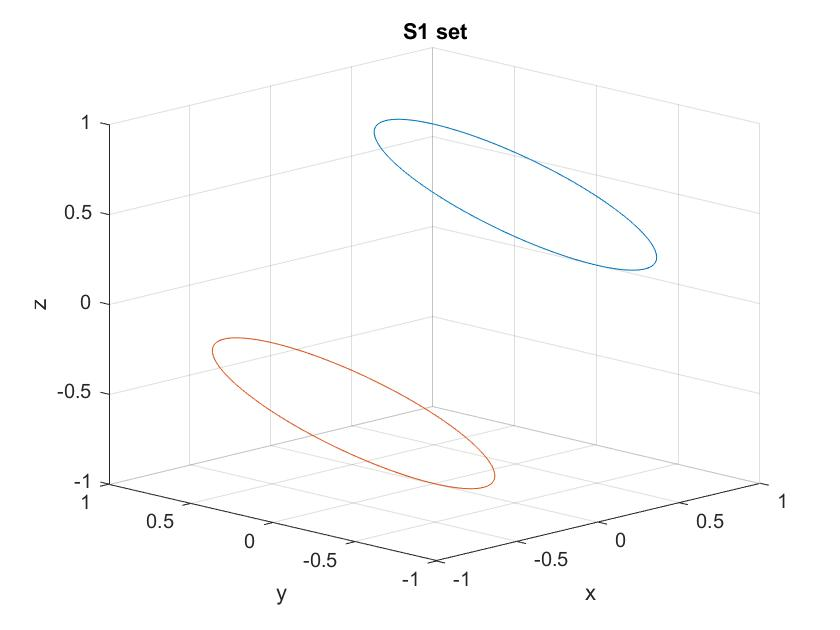
\includegraphics[width=0.8\textwidth]{41_circles.jpg}
        \captionof{figure}{Plot of $S_1$}
      \end{center}

      Now for the other set $S_2$. Since $M$ is symmetric, we have that the singular values are precisely the absolute values of the eigenvalues. Thus, $\lVert M \rVert_* \leq 1 \implies \lvert \lambda_1 \rvert + \lvert \lambda_2 \rvert \leq 1$. This gives us four inequalities, $\pm \lambda_1 + \pm \lambda_2 \leq 1$. We also have that
      \begin{gather*}
        \text{det}(M(x, y/\sqrt{2}, z) - \lambda I) = \lambda^2 - (x+z) \lambda + xz - y^2/2
      \end{gather*}
      Which means that the roots are
      \begin{gather*}
        \lambda = \frac{x+z \pm \sqrt{(x-z)^2 + 2y^2}}{2}
      \end{gather*}
      Combining these roots with the four inequalities before, we get the following inequalities
      \begin{gather*}
        -1 \leq x + z \leq 1 \\
        (x - z)^2 + 2 y^2 \leq 1
      \end{gather*}
      Using the same change of variable as before, these are equivalent to
      \begin{gather*}
        -1 \leq \sqrt{2} x' \leq 1 \\
        y'^2 + z'^2 \leq 1/2
      \end{gather*}
      Thus, this is a cylinder with axis (1,0,1) passing through the origin whose top and bottom line on the plane $x+z = \pm 1$ and radius $1/\sqrt{2}$. The plot is below.

      \begin{center}
        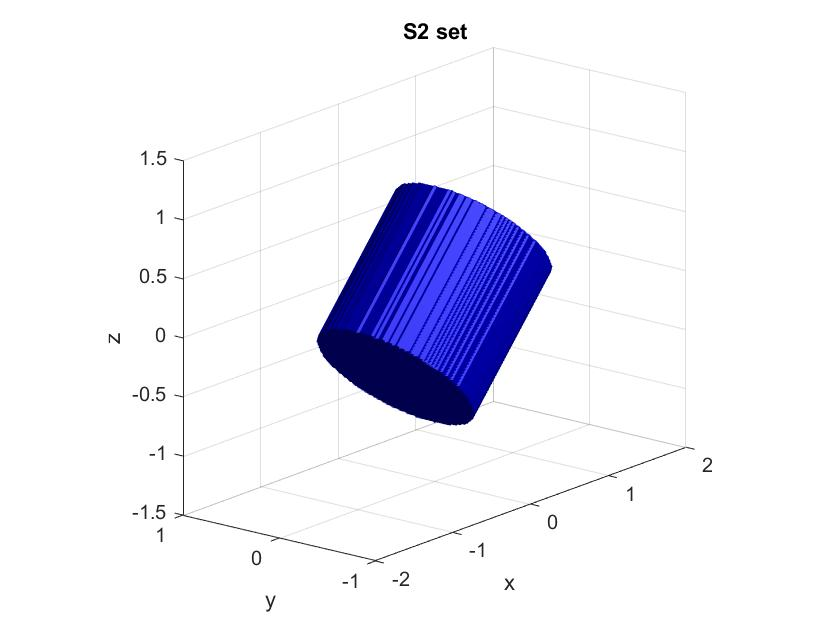
\includegraphics[width=0.8\textwidth]{41_cylinder.jpg}
        \captionof{figure}{Plot of $S_2$}
      \end{center}

    \item
      \begin{enumerate}[label=\alph*)]
        \item We show that both sides are less than or equal to each other to show equality. Let $U \Sigma V^T$ be the SVD of $Y$. Then, let $X = U V^T$. Their inner product is
          \begin{gather*}
            \langle Y, X \rangle = \text{trace}(V \Sigma U^T U V^T) \\
            = \text{trace}(V \Sigma I V^T) = \text{trace}(\Sigma V^T V) \\
            = \text{trace}(\Sigma) = \lVert Y \rVert_*
          \end{gather*}
          We also have that $\lVert X \rVert_{op} = 1$ since it is the largest singular value of $X$. Thus, we have showed $\lVert Y \rVert_* \leq \max_{X : \lVert X \rVert_{op} \leq 1} \langle Y, X \rangle$

          Now suppose that $\lVert X \rVert_{op} \leq 1$. Then
          \begin{gather*}
            \langle Y, X \rangle = \text{trace}(V \Sigma U^T X) = \text{trace}(U^T X V \Sigma)
          \end{gather*}
          We note that each operator norm for the matrices $U^T$ and $V$ are less than 1 since they are orthonormal and $X$ by assumption.
          \begin{gather*}
            \lVert U^T X V \rVert_{op} \leq \lVert U^T \rVert_{op} \lVert X \rVert_{op} \lVert V \rVert_{op} \leq 1
          \end{gather*}
          Now let $X' = U^T X V$, which makes the trace of $\langle Y, X \rangle$ equal to
          \begin{gather*}
            = \text{trace}(X' \Sigma) = \sum_{i=1}^n \sigma_i x'_{ii} \leq \sum_{i=1}^n \sigma_i \lvert x'_{ii} \rvert
          \end{gather*}
          But we just showed that $\lVert X' \rVert_{op} \leq 1$. Hence, we have
          \begin{gather*}
            = \text{trace}(X' \Sigma) \leq \sum_{i=1}^n \sigma_i = \lVert Y \rVert_*
          \end{gather*}
          So, $\max_{X : \lVert X \rVert_{op} \leq 1} \langle Y, X \rangle \leq \lVert Y \rVert_*$ and we conclude that
          \begin{gather*}
            \max_{X : \lVert X \rVert_{op} \leq 1} \langle Y, X \rangle = \lVert Y \rVert_*
          \end{gather*}

        \item Let $X, Y$ be matrices and $\lambda \in (0,1)$. Then
          \begin{gather*}
            \lVert \lambda X + (1-\lambda) Y \rVert_* = \max_{Z : \lVert Z \rVert_{op} \leq 1} \lambda \langle X, Z \rangle + (1-\lambda) \langle Y, Z \rangle \\
            \leq \lambda \max_{Z : \lVert Z \rVert_{op} \leq 1} \langle X, Z \rangle + (1-\lambda) \max_{Z : \lVert Z \rVert_{op} \leq 1} \langle Y, Z \rangle \\
            = \lambda \lVert X \rVert_* + (1-\lambda) \lVert Y \rVert_*
          \end{gather*}
          Therefore $\lVert \cdot \rVert_*$ is convex.

        \item Denote the sets by $A = \text{conv}\{ u v^T : \lVert u v^T \rVert_{op} \leq 1, u \in \mathbb{R}^{d_1}, v \in \mathbb{R}^{d_2} \}$ and $B = \{ X \in \mathbb{R}^{d_1 \times d_2}  : \lVert X \rVert_* \leq 1 \}$. We first show that $A \subseteq B$. From the previous part, $\lVert \cdot \rVert_*$ is convex, therefore $B$ is convex at it is a sublevel set of a convex function. Thus, we need not worry about the convex hull part and only need to show that $\forall u v^T$ with $\lVert u v^T \rVert_{op} \leq 1$, then $u v^T \in B$.

          We have that
          \begin{gather*}
            u v^T = \frac{u}{\lVert u \rVert} \lVert u \rVert \lVert v \rVert \frac{v^t}{\lVert v^T \rVert}
          \end{gather*}
          Where we assumed $u, v^T \neq 0$ because if they did, they are trivially in $B$. Thus, $\lVert u \rVert \lVert v \rVert$ is a non-zero singular calue of $u v^T$ as one can view the above as the SVD of $u v^T$. This gives us $\lVert u v^T \rVert_* = \lVert u \rVert \lVert v \rVert$. We then have
          \begin{gather*}
            \lVert u v^T \rVert_{op} = \max_i \sigma_i(u v^T) = \lVert u \rVert \lVert v^T \rVert = \lVert u v^T \rVert_*
          \end{gather*}
          However, we by assumption that the operator norm is bounded by 1and so the nuclear norm is bounded by 1, so we conclude that $u v^T \in B$.

          Now we show the other inclusion. First, define the SVD of $X = U \Sigma V^T$. If $X = 0$, then it is trivially in $A$. Assume $X \neq 0$, so that $\lVert X \rVert_* = \sum_{i=1}^d \sigma_i(X) > 0$. We first show that the $i^{th}$ columns of $U$ and $V$, $u_i v_i^T$, is in $A$. By Cauchy-Schwarz, for all $x \in \mathbb{R}^{d_2}$
          \begin{gather*}
            \lVert u_i v_i^T x \rVert \leq \lVert u_i \rVert \lVert v_i^T \rVert \lVert x \rVert = \lVert x \rVert
          \end{gather*}
          Thus, we have that $u_i v_i^T \in A$. Now, we rewrite $X$ as follow which is the SVD in summation form
          \begin{gather*}
            X = \sum_{i=1}^d \frac{\sigma_i}{\sum_{i=1}^d \sigma_i} (u_i v_i^T \sum_{i=1}^d \sigma_i)
          \end{gather*}
          But, since $\sum_{i=1}^d \sigma_i$ by assumption, we have $(u_i v_i^T \sum_{i=1}^d \sigma_i) \in A$. Then the outer sum is a convex combination of element in $A$, thus it is also in $A$. So we showed that $X \in A$ and $B \subseteq A$. We conclude that $A = B$.
      \end{enumerate}

    \item Starting with the objective, we first do the SVD decomposition for $X$. Then, we use the hint and use the fact that the Frobenius norm is invariant under unitary transforms.
      \begin{gather*}
        \lVert Z \rVert_* + \frac{\tau}{2} \lVert X - X Z \rVert_F^2 \\
        = \lVert Z \rVert_* + \frac{\tau}{2} \lVert U \Lambda V^T - U \Lambda V^T Z \rVert_F^2 \\
        = \lVert Z \rVert_* + \frac{\tau}{2} \lVert \Lambda V^T - \Lambda V^T Z \rVert_F^2 \\
        = \lVert Z \rVert_* + \frac{\tau}{2} \lVert \Lambda - \Lambda V^T Z V \rVert_F^2
      \end{gather*}
      Since $V$ is unitary, then there is a one-to-one correspondence between $Z$ and $V^T Z V$ and we can focus on solving
      \begin{gather*}
        \min_Z \lVert Z \rVert_* + \frac{\tau}{2} \lVert \Lambda - \Lambda Z \rVert_F^2
      \end{gather*}
      We first handle the case when $Z$ is diagonal. Let $Z = \Lambda_Z = \text{diag}(\lambda_{z_i})$. Then the objective becomes
      \begin{gather*}
        \lVert \Lambda_Z \rVert_* + \frac{\tau}{2} \lVert \Lambda - \Lambda \Lambda_Z \rVert_F^2 \\
        \sum_{i=1}^d \lvert \lambda_{z_i} \rvert + \frac{\tau}{2} \sum_{i=1}^d \lambda_i^2 (1-\lambda_{z_i})^2
      \end{gather*}
      Thus, we get lower values when $\lambda_{z_i} \geq 0$, so we take $\Lambda \succeq 0$. Which turns the minimization problem into
      \begin{gather*}
        \min_{\lambda_{z_i} \geq 0} \sum_{i=1}^d \lvert \lambda_{z_i} \rvert + \frac{\tau}{2} \sum_{i=1}^d \lambda_i^2 (1-\lambda_{z_i})^2
      \end{gather*}
      This is a convex optimization problem. Slater's condition also guarantees that KKT conditions are necessary and sufficient. We then have that there exists $\mu \geq 0$ s.t.
      \begin{gather*}
        - \tau \lambda_i^2 (1-\lambda_{z_i}) + 1 - \mu_i = 0 \\
        \Longleftrightarrow \tau \lambda_i^2 \lambda_{z_i} - \tau \lambda_i^2 + 1 = \mu_i \geq 0
      \end{gather*}
      and our slackness conditions
      \begin{gather*}
        \mu_i \lambda_{z_i} = 0 \ \forall i
      \end{gather*}
      Now we handle a couple of cases. Suppose $\tau \lambda_i^2 - 1 > 0$. Then if $\mu_i > 0$, $\lambda_{z_i} = 0$ by slackness, and so $\mu_i = -\tau \lambda_i^2 + 1 < 0$ which is a contradiction. Thus, we have
      \begin{gather*}
        \mu_i = 0 \\
        \lambda_{z_i} = 1 - \frac{1}{\tau} \lambda_i^{-2} > 0
      \end{gather*}
      If $\tau \lambda_i^2 - 1 \leq 0$, then $\lambda_{z_i} = 0$ since if it strictly positive, then $\mu_i > 0$ which fails slackness. Thus, $\lambda_{z_i} = 0$. Therefore, we have shown for a diagonal matrix $Z$, we have that the minimizer is $\max (0, I - \frac{1}{\tau} \Lambda^{-2})$.

      Now, if we can show that the solution must be a diagonal, then we are done. We begin by showing that $\lvert A \rVert_* \geq \lVert \text{diag}(A) \rVert_* \ \forall A$. We have that
      \begin{gather*}
        \lVert \text{diag}(A) \rVert_* = \sum_{i=1}^d \lvert a_{ii} \rvert \text{ and } \\
        \lVert A \rVert_* = \max_{X : \lVert X \rVert_{op} \leq 1} \langle A, X \rangle
      \end{gather*}
      Now construct $X$ to be diagonal with $x_{ii} = $ sign($a_{ii}$). This yields
      \begin{gather*}
        \lVert X \rVert_{op} \leq 1 \text{ and } \langle A, X \rangle = \lVert \text{diag}(A) \rVert_*
      \end{gather*}
      Thus we conclude that $\lvert A \rVert_* \geq \lVert \text{diag}(A) \rVert_* \ \forall A$. Thus, if we find a solution $Z$, then we can decrease the nuclear norm of the minimization by simply taking the diag($Z$) instead to be our solution. Lets see what happens to the Frobenius norm.
      \begin{gather*}
        \lVert \Lambda - \Lambda Z \rVert_F^2 \\
        = \text{trace}((\Lambda - \Lambda Z)^T(\Lambda - \Lambda Z)) \\
        = \text{trace}( \Lambda^2 - Z^T \Lambda^2 - \Lambda^2 Z + Z^T \Lambda^2 Z ) \\
        = \text{trace}(\Lambda^2) - 2*\text{trace}(\Lambda^2 Z) + \text{trace}(\Lambda^2 Z Z^T) \\
        = \text{trace}(\Lambda^2) - 2*\text{trace}(\Lambda^2 \text{diag}(Z)) + \lVert \Lambda Z \rVert_F^2 \\
        \geq \text{trace}(\Lambda^2) - 2*\text{trace}(\Lambda^2 \text{diag}(Z)) + \lVert \Lambda \text{diag}(Z) \rVert_F^2
      \end{gather*}
      Thus, by taking $Z$ to be the diag($Z$), then we see that the Frobenius norm does not change since $\Lambda^2$ is diagonal. The first term has no $Z$, the middle term will be unchanged, and the last term is $\lVert \Lambda Z \rVert_F^2$ whose singular values do not increase since $\Lambda^2$ is positive and diagonal. That is, for every $Z$, we can find a diagonal matrix that is at least as good as it. Thus, we conclude that all solutions will be diagonal and so we have shown that
      \begin{gather*}
        \widehat{Z} = V \max (0, I - \frac{1}{\tau} \Lambda^{-2}) V^T
      \end{gather*}
      is the optimal solution to the optimization problem.
  \end{enumerate}
\end{answer}

\clearpage

\begin{exercise}
  Consider
  \begin{gather*}
    \min_\beta \frac{1}{2} \lVert Y - X \beta \rVert_2^2 + \lambda \lVert \beta \rVert_1
  \end{gather*}
  \begin{enumerate}[label=\arabic*)]
    \item If $\widehat{\beta}_1$ and $\widehat{\beta}_2$ are both minimizers of the above problem, prove they have the same prediction $X \widehat{\beta}_1 = X \widehat{\beta}_2$. This result suggests that even the Lasso solution may not be unique, linear predictors based on them turn out to be unique!

      (\textbf{Hint:} Consider the vector $\alpha \widehat{\beta}_1 + (1-\alpha) \widehat{\beta}_2$ for $\alpha \in (0,1)$.)

    \item Let $\widehat{\beta}$ be a minimizer for the above problem. Denote $X_j$ to be the $j^{th}$ column of $X$, prove that
      \begin{gather*}
        \begin{cases}
          \lambda = X_j^T(Y - X \widehat{\beta}) & \text{ if } \widehat{\beta}_j > 0 \\
          \lambda = -X_j^T(Y - X \widehat{\beta}) & \text{ if } \widehat{\beta}_j < 0 \\
          \lambda \geq \lvert X_j^T(Y - X \widehat{\beta}) \rvert & \text{ if } \widehat{\beta}_j = 0
        \end{cases}
      \end{gather*}

      (\textbf{Hint:} If $x^*$ minimizes a convex function $f(x)$, if and only if $0 \in \partial f(x^*)$. You can directly use this and the subgradient of $\ell_1$ norm.)

    \item If $\lambda > \lVert X^T Y \rVert_\infty$, where $\lVert \cdot \rVert_\infty$ is the sup-norm, prove that the minimizer of the above minimization must be zero.

      (\textbf{Hint:} User Q4.1 and Q4.2.)

    \item Suppose the problem above has a unique minimizer for all $\lambda > 0$, denoted by $\widehat{\beta}(\lambda)$. Given $[\lambda_0, \lambda_1]$, suppose the support and the signs of $\widehat{\beta}(\lambda)$ are unchanged for $\lambda_0 \leq \lambda \leq \lambda_1$. Show that there is a vector $\gamma_0$ such that
      \begin{gather*}
        \widehat{\beta}(\lambda) = \widehat{\beta}(\lambda_0) - (\lambda - \lambda_0)\gamma_0
      \end{gather*}
      This result proves that the Lasso regularization path is piecewise linear!! Compare the result with the Lasso regularization path in Q1.3 and explain why that plot is also piecewise linear (Note, the horizontal axis in that plot is $\lVert \beta \rVert_1$?)

      (\textbf{Hint:} Use Q4.2. You may need the Moore-Penrose pseudoinverse. Given a SVD of rank $r$ matrix $A = U \Lambda V^T \in \mathbb{R}^{n \times d}$, where $U \in \mathbb{R}^{n \times r}$, $V \in \mathbb{R}^{d \times r}$. The pseudoinverse of $A$ is $A^\dagger = V \Lambda^{-1} U^T$.)

    \item Consider the design such that $X \in \mathbb{R}^{n \times d}$ with Rank($X$) $= n$. We again suppose $\widehat{\beta}(\lambda)$ is the unique minimizer of the optimization problem above for all $\lambda > 0$. Prove that when $\lambda$ goes to zero, the Lasso estimator converges to one of the compressed sensing estimator
      \begin{gather*}
        \widehat{\beta}^{CS} = \argmin_{\beta} \lVert \beta \rVert_1 \text{ s.t. } Y = X \beta
      \end{gather*}
      Namely, prove that there exists a solution of the above problem $\widehat{\beta}^{CS}$ such that
      \begin{gather*}
        \lim_{\lambda \rightarrow 0^+} \widehat{\beta}{\lambda} = \widehat{\beta}^{CS}
      \end{gather*}

      (\textbf{Hint:} You may need to first prove the existence of the limitation by bounding the number of piecewise lines in Q4.4.)
  \end{enumerate}
\end{exercise}

\begin{answer}
  \begin{enumerate}[label=\arabic*)]
    \item Note that $X \widehat{\beta}$ is a vector. Thus, consider the vector function $f(X) = \frac{1}{2}\lVert Y - X \rVert_2^2$. Then we have
      \begin{gather*}
        \nabla f(X) = X - Y \\
        \nabla^2 f(X) = I \succ 0
      \end{gather*}
      That is, $f(X)$ is strictly convex. Thus, $\frac{1}{2} \lVert Y - X \beta \rVert_2^2 + \lambda \lVert \beta \rVert_1$ is a strictly convex function plus a convex function. This results in a strictly convex function. Now, take any two optimal $X \widehat{\beta}_1$ and $X \widehat{\beta}_2$ and suppose they are not equal. We will show that we they cannot be optimal. Let $f(X)$ be as before and $g(X) = \lVert X \rVert_1$. Take a convex combination of these vectors,
      \begin{gather*}
        f(\alpha X \widehat{\beta}_1 + (1-\alpha) X \widehat{\beta}_2) + g(\alpha X \widehat{\beta}_1 + (1-\alpha)X \widehat{\beta}_2)
      \end{gather*}
      By strict convexity of $f$ and convexity of $g$
      \begin{gather*}
        < \alpha f( X \widehat{\beta}_1) + (1-\alpha) f(X \widehat{\beta}_2) + \alpha g( X \widehat{\beta}_1) + (1-\alpha) g(X \widehat{\beta}_2)
      \end{gather*}
      However, this shows that $\alpha X \widehat{\beta}_1 + (1-\alpha) X \widehat{\beta}_2$ is more optimal than $X \widehat{\beta}_1$ and $X \widehat{\beta}_2$ which contradicts the assumption that they were optimal. Therefore, we must have that $X \widehat{\beta}_1 = X \widehat{\beta}_2$.

    \item We have $f$ and $g$ as defined in the last part. The subgradient of the problem is
      \begin{gather*}
        \partial (f+g) = -X^T(Y - X \beta) + \lambda \partial g
      \end{gather*}
      We have that $a \in \partial g(\beta)$ if for all $\gamma$
      \begin{gather*}
        \lVert \gamma \rVert_1 - \lVert \beta \rVert_1 \geq a^T (\gamma - \beta) \\
        \sum_{j=1}^n \lvert \gamma_j \rvert - \lvert \beta_j \rvert \geq a_j^T (\gamma_j - \beta_i)
      \end{gather*}
      That is, we require that $a_j \in \partial \lvert \beta_j \rvert$ for all $j$. This is much easier to see that
      \begin{gather*}
        a_j \in \partial \lvert \beta_j \rvert = \begin{cases}
          \{1\} & \text{ if } \beta_j > 0 \\
          \{-1\} & \text{ if } \beta_j < 0 \\
          [-1,1] & \text{ if } \beta_j = 0
        \end{cases}
      \end{gather*}
      Thus, we have that $a \in \partial \lVert \beta \rVert_1 = g$ if for all $j$
      \begin{gather*}
        a \in \partial \lvert \beta_j \rvert = \begin{cases}
          \{1\} & \text{ if } \beta_j > 0 \\
          \{-1\} & \text{ if } \beta_j < 0 \\
          [-1,1] & \text{ if } \beta_j = 0
        \end{cases}
      \end{gather*}
      This means that $0 \in \partial (f+g)$ iff $X^T(Y - X \beta) \in \lambda \partial g = \lambda \partial \lVert \beta \rVert_1$. Equivalently, for all $j$,
      \begin{gather*}
        \begin{cases}
          \lambda = X_j^T(Y - X \beta) & \text{ if } \beta_j > 0 \\
          \lambda = -X_j^T(Y - X \beta) & \text{ if } \beta_j < 0 \\
          \lambda \geq \lvert X_j^T(Y - X \beta) \rvert & \text{ if } \beta_j = 0
        \end{cases}
      \end{gather*}

    \item We will show that $\lambda \geq \lvert X_j^T(Y - X \beta) \rvert$ to conclude that $\beta_j = 0$ by part Q4.2.
      \begin{gather*}
        \lambda > \lVert X^T Y \rVert_\infty \geq \lvert X_j^T Y \rvert \ \forall j
      \end{gather*}
      However, note that if $\beta = 0$, we have that $X \beta = 0$, and so
      \begin{gather*}
        \lvert X_j^T Y \rvert = \lvert X_j^T (Y - X \beta) \rvert \ \forall j
      \end{gather*}
      That is, if $\beta = 0$,
      \begin{gather*}
        \lambda > \lvert X_j^T (Y - X \beta) \rvert \ \forall j
      \end{gather*}
      And by Q4.2, we have that $\widehat{\beta} = 0$ is an optimal solution. By Q4.1, we have that two optimal solutions have the same prediction. That is $X \widehat{\beta_1} = X \widehat{\beta_2}$. However, we showed $\widehat{\beta_1} = 0$ is optimal and the optimal value is $\frac{1}{2}\lVert Y \rVert_2^2$. So, $X \widehat{\beta_2} = 0$. This implies that
      \begin{gather*}
        \frac{1}{2} \lVert Y - X \widehat{\beta}_2 \rVert_2^2 + \lambda \lVert \widehat{\beta}_2 \rVert_1 = \frac{1}{2}\lVert Y \rVert_2^2 \\
        \implies \lambda \lVert \widehat{\beta}_2 = 0
      \end{gather*}
      Since $\lambda > 0$, we conclude that $\widehat{\beta}_2 = 0$ and so $\widehat{\beta} = 0$ is unique.

    \item A good guess for $\gamma_0$ is the linear interpolation between the end points $\widehat{\beta}(\lambda_1)$ and $\widehat{\beta}(\lambda_0)$. That is
      \begin{gather*}
        \gamma_0 = \frac{\widehat{\beta}(\lambda_1) - \widehat{\beta}(\lambda_0)}{\lambda_0 - \lambda_1}
      \end{gather*}
      We then wish to show that
      \begin{gather*}
        f(\lambda) = \widehat{\beta}(\lambda_0) - (\lambda - \lambda_0) \gamma_0 \\
        = \frac{\lambda_1 - \lambda}{\lambda_1 - \lambda_0} \widehat{\beta}(\lambda_0) + \frac{\lambda - \lambda_0}{\lambda_1 - \lambda_0} \widehat{\beta}(\lambda_1)
      \end{gather*}
      Satisfies the optimality conditions in Q4.2. Notice that we have
      \begin{gather*}
        \begin{cases}
          \widehat{\beta}_i > 0 \Leftrightarrow f(\lambda)_i > 0 \\
          \widehat{\beta}_i < 0 \Leftrightarrow f(\lambda)_i < 0 \\
          \widehat{\beta}_i = 0 \Leftrightarrow f(\lambda)_i = 0
        \end{cases}
      \end{gather*}
      Then let $I_-$, $I_0$, and $I_+$ denote the set of indices that are negative, zero, and positive respectively. Now, for $i \in I_+$, we have $f(\lambda)_i > 0$. Then we have
      \begin{gather*}
        X_j^T (Y - X f(\lambda)) = \frac{\lambda_1 - \lambda}{\lambda_1 - \lambda_0} X_j^T (Y - X \widehat{\beta}(\lambda_0)) + \frac{\lambda - \lambda_0}{\lambda_1 - \lambda_0} X_j^T (Y - X \widehat{\beta}(\lambda_1))
      \end{gather*}
      Now note that $\lambda_1 = X_j^T (Y - X \widehat{\beta}(\lambda_1))$ and $\lambda_0 = X_j^T (Y - X \widehat{\beta}(\lambda_0))$. So,
      \begin{gather*}
        = \frac{\lambda_1 - \lambda}{\lambda_1 - \lambda_0} \lambda_0 + \frac{\lambda - \lambda_0}{\lambda_1 - \lambda_0} \lambda_1 = \lambda
      \end{gather*}
      Thus, $f(\lambda)$ is optimal in the set of indices $I_+$. A similar sequence of computation follows for $I_-$. The case $I_0$ is different. Thus, we have that $\lambda_1 \geq \lvert X_j^T (Y-X \widehat{\beta}(\lambda_1)) \rvert$ and $\lambda_0 \geq \lvert X_j^T (Y-X \widehat{\beta}(\lambda_0)) \rvert$. Working in the oppositive direction as $I_+$ we get
      \begin{gather*}
        \lambda = \frac{\lambda_1 - \lambda}{\lambda_1 - \lambda_0} \lambda_0 + \frac{\lambda - \lambda_0}{\lambda_1 - \lambda_0} \lambda_1 \\
        \geq \frac{\lambda_1 - \lambda}{\lambda_1 - \lambda_0} \lvert X_j^T (Y - X \widehat{\beta}(\lambda_0)) \rvert + \frac{\lambda - \lambda_0}{\lambda_1 - \lambda_0} \lvert X_j^T (Y - X \widehat{\beta}(\lambda_1)) \rvert \\
        \geq \lvert X_j^T (Y - X (\frac{\lambda - \lambda_0}{\lambda_1 - \lambda_0}\widehat{\beta}(\lambda_1) +  \frac{\lambda_1 - \lambda}{\lambda_1 - \lambda_0}\widehat{\beta}(\lambda_0))) \rvert \\
        = \lvert X_j^T (Y - X f(\lambda)) \rvert
      \end{gather*}
      Where we used the triangle inequality to combine the absolute values. Thus, $f(\lambda)$ is an optimal solution for all $\lambda \in [\lambda_0, \lambda_1]$. By assumption, there is a unique minimizer. Thus,
      \begin{gather*}
        \widehat{\beta}(\lambda) = f(\lambda) = \widehat{\beta}(\lambda_0) - (\lambda - \lambda_0) \gamma_0
      \end{gather*}
      The Lasso regularization path in Q1.3 was also piecewise linear and has to do with the fact that if $\widehat{\beta}(\lambda)$ is piecewise linear, then we have that the L1 norm is a sum of piecewise linear functions which is piecewise linear.

    \item One can argue that $\lim_{\lambda \rightarrow 0+} \widehat{\beta}(\lambda)$ converges because it is a sequence of piece wise linear functions. That is, there will be small interval $(0,\epsilon)$ for $\epsilon$ sufficiently small, that the $\widehat{\beta}(\lambda)$ will be linear on. This is justified by the fact that there is only a finite number of intervals that $\widehat{\beta}(\lambda)$ is linear on due to the fact that there is only a finite number of indices.
  \end{enumerate}
\end{answer}

\end{document}